\providecommand{\main}{..}
\documentclass[\main/master.tex]{subfiles}
\begin{document}
\chapter{Another Example Chapter}\label{chp:example-2}
\hspace{5 mm} This another example chapter with a working reference as see in Chapter~\ref{chp:example-1}. There I also made an example of an equation, see Eqn.~\ref{eqn:energy-mass-equivalence-relation}. We also created an example image, see Fig.~\ref{fig:sine-wave}.
\begin{figure}[htbp]
	\centering
	\fbox{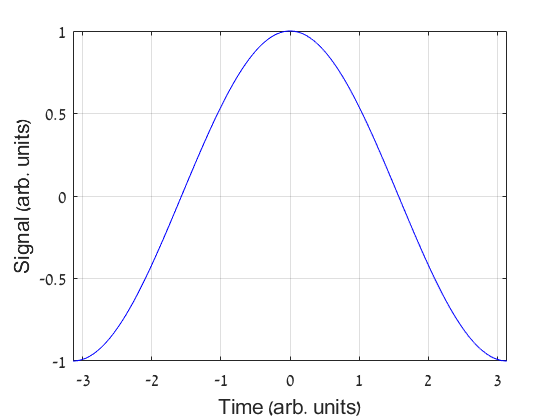
\includegraphics[scale=0.75]{\main/images/chapter_2_example/img_example_2.png}}
	\caption[Another Example Image]{Another Example Image. This image is also labeled internally so we can referenc it throughout the text.}
	\label{fig:sine-wave}
\end{figure}
\end{document}